\documentclass{article}



\usepackage{arxiv}

\usepackage[utf8]{inputenc} % allow utf-8 input
\usepackage[T1]{fontenc}    % use 8-bit T1 fonts
\usepackage{hyperref}       % hyperlinks
\usepackage{url}            % simple URL typesetting
\usepackage{booktabs}       % professional-quality tables
\usepackage{amsfonts}       % blackboard math symbols
\usepackage{nicefrac}       % compact symbols for 1/2, etc.
\usepackage{microtype}      % microtypography
\usepackage{lipsum}		% Can be removed after putting your text content
\usepackage{graphicx}
\usepackage[numbers]{natbib}
\usepackage{subcaption}

\usepackage{doi}



\title{Experimental Analysis of MCMF problem}

\date{June 30, 2021}	% Here you can change the date presented in the paper title
%\date{} 					% Or removing it

\author{ \href{https://orcid.org/0000-0003-3730-6778}{
\includegraphics[scale=0.06]{orcid.pdf}\hspace{1mm}Anirudha~Kulkarni}\thanks{Webpage: \href{https://anirudhakulkarni.github.io}{https://anirudhakulkarni.github.io}} \\
	Department of Computer Science and Engineering\\
	Indian Institute of Technology Delhi\\
	New Delhi - 110016, India\\
	\texttt{cs5190421@iitd.ac.in} \\
	%% examples of more authors
% 	\And
% 	\href{https://orcid.org/0000-0000-0000-0000}{
\includegraphics[scale=0.06]{orcid.pdf}\hspace{1mm}Elias D.~Striatum} \\
% 	Department of Electrical Engineering\\
% 	Mount-Sheikh University\\
% 	Santa Narimana, Levand \\
% 	\texttt{stariate@ee.mount-sheikh.edu} \\
    \\
    \AND
    \textbf{Guided By:}\\
	\href{https://orcid.org/0000-0002-5476-8328}{
\includegraphics[scale=0.06]{orcid.pdf}\hspace{1mm}\textbf{Prof. Sathish~Vadhiyar}}\thanks{Webpage: \href{http://cds.iisc.ac.in/faculty/vss/}{http://cds.iisc.ac.in/faculty/vss/}} \\
	Department of Computational and Data Sciences\\
	Indian Institute of Science\\
	Bangalore-560012, India\\
    \texttt{vss@cds.iisc.ac.in} \\
	%% \And
	%% Coauthor \\
	%% Affiliation \\
	%% Address \\
	%% \texttt{email} \\
	%% \And
	%% Coauthor \\
	%% Affiliation \\
	%% Address \\
	%% \texttt{email} \\
}

% Uncomment to remove the date
%\date{}

% Uncomment to override  the `A preprint' in the header
\renewcommand{\headeright}{4 Week Report}
\renewcommand{\undertitle}{4 Week Report}
\renewcommand{\shorttitle}{Experimental Analysis of MCMF problem}

%%% Add PDF metadata to help others organize their library
%%% Once the PDF is generated, you can check the metadata with
%%% $ pdfinfo template.pdf
\hypersetup{
pdftitle={Experimental Analysis of MCMF problem},
pdfsubject={q-bio.NC, q-bio.QM},
pdfauthor={Anirudha~Kulkarni},
pdfkeywords={First keyword, Second keyword, More},
}

\begin{document}
\maketitle

\begin{abstract}
Network flows models a large variety of problems across computer science, transportation and mathematics. A flow which is maximum possible in given constraints and with minimum possible cost solves majority of the problems. There are many different algorithms to do so, but most of them are inherently sequential. As networks get large which is the case in many real-life applications, these algorithms are not practical to use. With driver problem of finding optimal distribution of oxygen from factories to districts across country, We investigate the various ways to solve the problem and investigate how much speedup can be obtained with these algorithms due to parallelism.


\end{abstract}


% keywords can be removed
\keywords{MCMF \and Network Simplex \and Cost Scaling}


\section{Introduction}
Network flows models a large variety of problems. Given sources and sinks, the flow is a fundamental characteristic of the network. Optimizing such a flow against constraints of a network has wide range of applications in various fields ranging from transportation, scheduling, resources planning to telecommunication. Minimum cost flow problem (MCF) plays important role in optimization of such a flow in cost constrained environment.

Given the fact that in recent months India saw heavy shortage of oxygen having three times more supply than actual demand on peak days of the crisis \citep{BBC}, we chose this as our driver problem. This motivated us to model the factories across country and hospitals to find optimal distribution which will lead to lowest cost in terms of finances and time delay.

In section 2 we will describe the problem and various algorithms to solve them. section 3 consist of market research and methodology. We will discuss the results in section 4 and future work in section 5.
\section{Background}

\subsection{MCMF: Minimum Cost Maximum Flow}

A flow network is a directed graph $G=(V,E)$ with a source vertex $s \in V$ and a sink vertex $t \in V$, where each edge $(u,v) \in E$ has capacity $c(u,v) > 0$, flow $f(u,v) \ge 0$ and cost $a(u,v)$. The cost of sending a flow along an edge $(u,v)$ is defined as $f(u,v)\cdot a(u,v)$. The problem requires maximising the amount of flow $d$ to be sent from source $s$ to sink $t$ and minimize the \textbf{total cost} of the flow over all edges given by:

\[\sum_{(u,v) \in E} a(u,v) \cdot f(u,v)\]
With the constraints:
% \begin{gather}

\[\textbf{Capacity constraints:}  \,f(u,v) \le c(u,v)\]
\[\textbf{Skew symmetry:} \,f(u,v) = - f(v,u)\]
\[\textbf{Flow conservation:}  \,\sum_{w \in V} f(u,w) = 0 \textit{ for all } u \neq s, t\]
\[\textbf{Required flow:}  \,\sum_{w \in V} f(s,w) = d \textit{ and } \sum_{w \in V} f(w,t) = d\]
% \end{gather}

\subsection{Modeling with MCMF}
To model the problem, we represent source factories as source nodes and district as sink nodes in a flow network. For each source node we add an arch of infinite capacity and weight of distance from source to each district. We then add super-source and super-sink which acts as only "Source" and only "Sink" in MCMF problem. For each source we add edge from super-source to source with zero weight and capacity equal to capacity of the source node. Similarly we add edge corresponding to each sink to super-sink with zero weight and capacity as demand of sink node. We make changes in this model as per algorithm requirements.

\begin{figure}[h]
\centering
  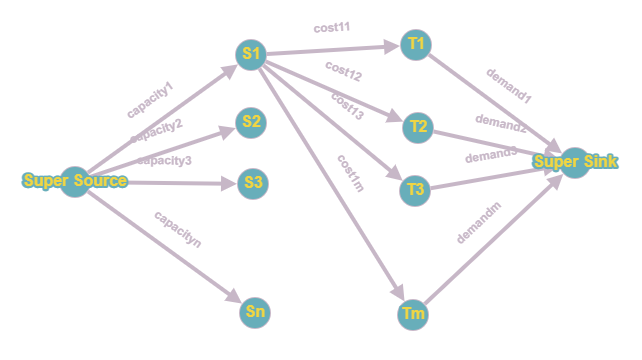
\includegraphics[width=0.6\linewidth]{model.png}
\label{fig:sub1}
\caption{Modeling Problem as MCMF problem }
\label{fig:test}
\end{figure}

\section{Market Research}
We found three most used libraries to solve this problem: \emph{Networkx}, \emph{Boost Graph Library}, \emph{LEMON}
\subsection{Networkx}
Networkx is a python library for graphs and networks. It provides $network\_simplex()$ and $max\_flow\_min\_cost()$ functions to solve the MCMF problem. Both are implementation of Network simplex algorithm \cite{kiraly2012efficient} but differ in implementation. Minimum cost maximum flow algorithm require only cost and weight of the edges augmented with source capacities and sink demands. It calculates maximum flow possible through the network given infinite capacity of super-source. This might sound as limitation and question relevance in real life example where infinite source is not possible but as we have already augmented the source production capacity as capacity of edge, there can not be a flow more than source capacity through the source node. 

Network simplex algorithm require the super-source capacity and super-sink demand to be mentioned and be exactly same. For this we calculate demand of all sink nodes and provide it as capacity of super-source node. This will again not violet the maximum flow that can flow through source nodes due to restriction imposed by edge capacities.
\subsection{Boost Graph Library}
Boost Graph Library is subset of well known boost library for graphs. It provides generic interface similar to Standard Template Library (STL) that allows access to a graph's structure, but hides the details of the implementation. 


Boost provides \emph{successive\_shortest\_path\_nonnegative\_weights()}.
The function calculates the flow values $f(u,v)$ for all $(u,v) \in E$, which are returned in the form of the residual capacity $r(u,v) = c(u,v) - f(u,v)$. It requires the directed graph $G=(V,E)$ that represents the network to be augmented to include the reverse edge for every edge in $E$. Hence the input graph become $G_{in} = (V,\{E \cup E^{T}\})$. 

Also, the capacity of each edge in $E$ to a positive number, and each edge in $E_T$ is $0$. The weight of each edge from $E$ must be a non-negative number, and each edge from $E_T$ must be $-weight$ of its reversed edge. Supplementary function \emph{find\_flow\_cost()} can be used to find the cost of the resulted flow.
\subsection{LEMON : Library for Efficient Modeling and Optimization in Networks}
LEMON stands for Library for Efficient Modeling and Optimization in Networks. It is a C++ template library providing efficient implementations of data structures and algorithms with support for optimization problems on graphs and networks. LEMON provides several implementation for MCMF problem. Previous work suggest that cost-scaling and primal network simplex algorithms performs significantly better than other implementations\citep{doi:10.1080/10556788.2014.895828}. So we chose them for our analysis.
% \section{Methodology}
% \label{sec:headings}

\section{Experimental Setup}
We used Intel Xenon 32 cores CPU ES-26700 @2.60GHz with 130 GB RAM. To get maximum performance we distributed the various iterations over multiple cores but each iteration was kept sequential. We used production data provided by All India Industrial Gases Manufacturer’s Association to generate graph with required production capacities. For demand we distributed the net supply among all districts due to lack of data. This gave worst case runtime on given number of nodes.

\subsection{Project OSRM - Distance API}
We used Project OSRM free APIs to calculate distance by car between two locations.
Project OSRM is  Modern C++ routing engine for shortest paths in road networks. It provides on road distance between two locations. Its free version allows approximately 2 JSON based API calls per second which becomes bottleneck in large scale graphs.  

\section{Results and Discussion}
\subsection{Networkx}
We found the runtime of the algorithms by varying number of source nodes and sink nodes. Network simplex algorithm performs significantly faster than Maximum flow Minimum cost algorithm. For our driver problem we considered worst case scenario where we had 742 total nodes with 371 source nodes and 371 sink nodes. It took less than 2 minutes with maximum cost minimum flow algorithm and less than 10 seconds for Network simplex algorithm. 
% \autoref{fig:test}
\begin{figure}[h]
\centering
\begin{subfigure}{0.5\textwidth}
  \centering
  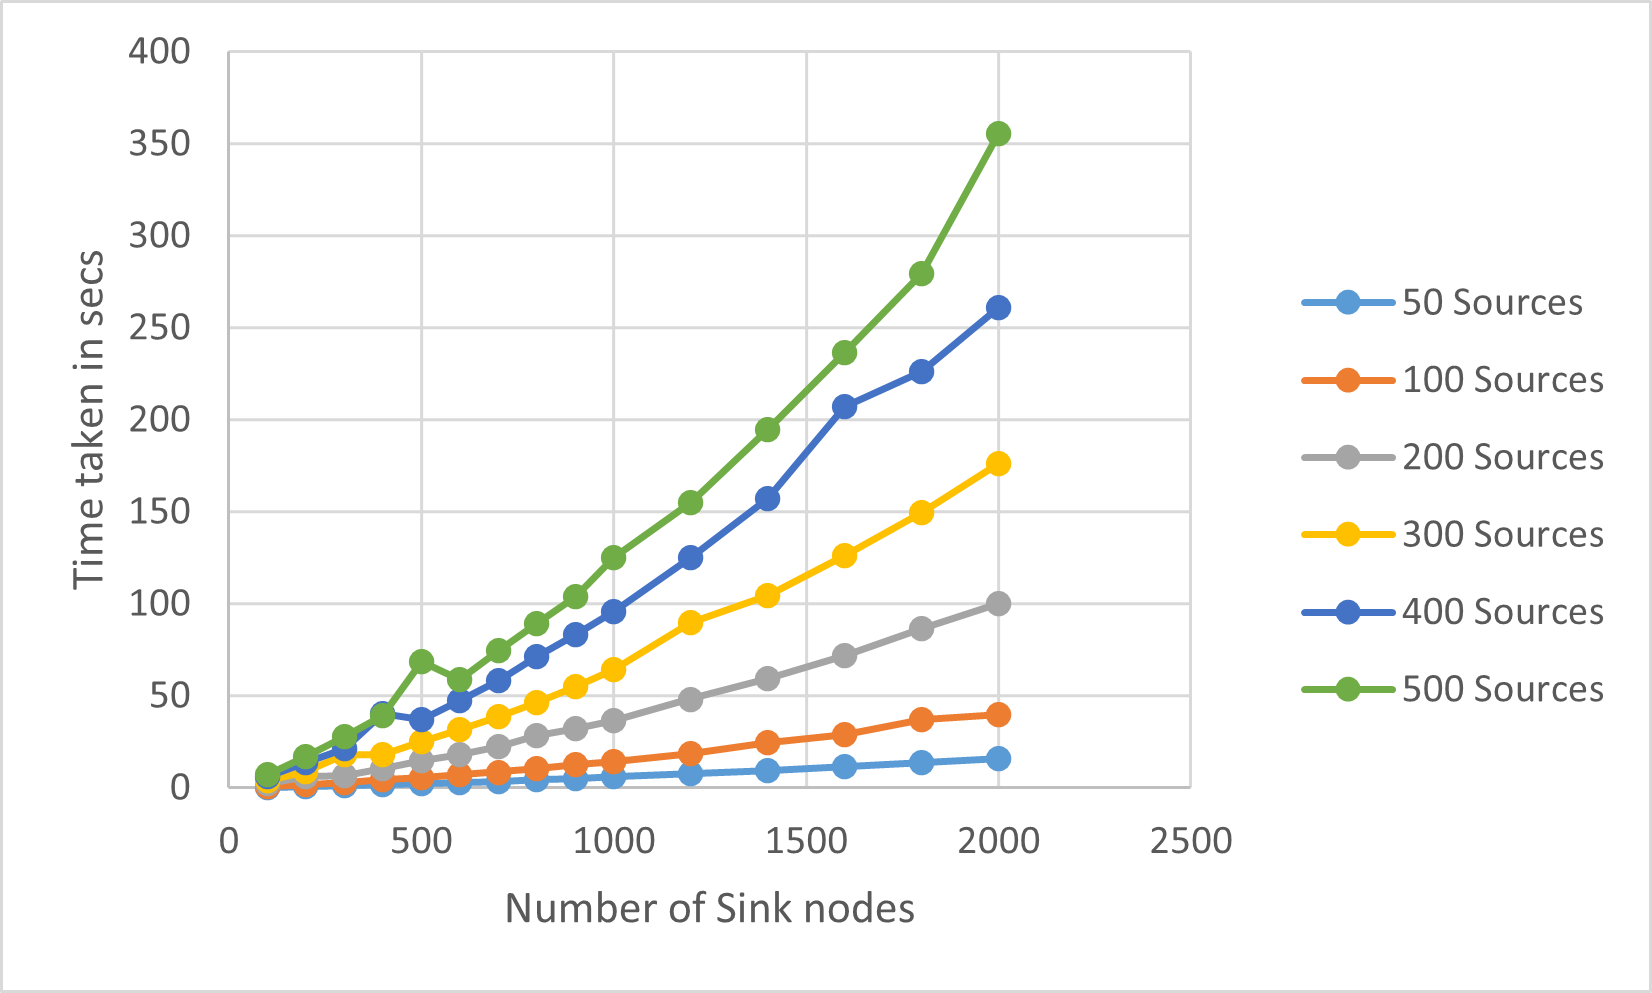
\includegraphics[width=0.9\linewidth]{mcmf.png}
  \caption{$max\_flow\_min\_cost()$ function}
  \label{fig:sub1}
\end{subfigure}%
\begin{subfigure}{0.5\textwidth}
  \centering
  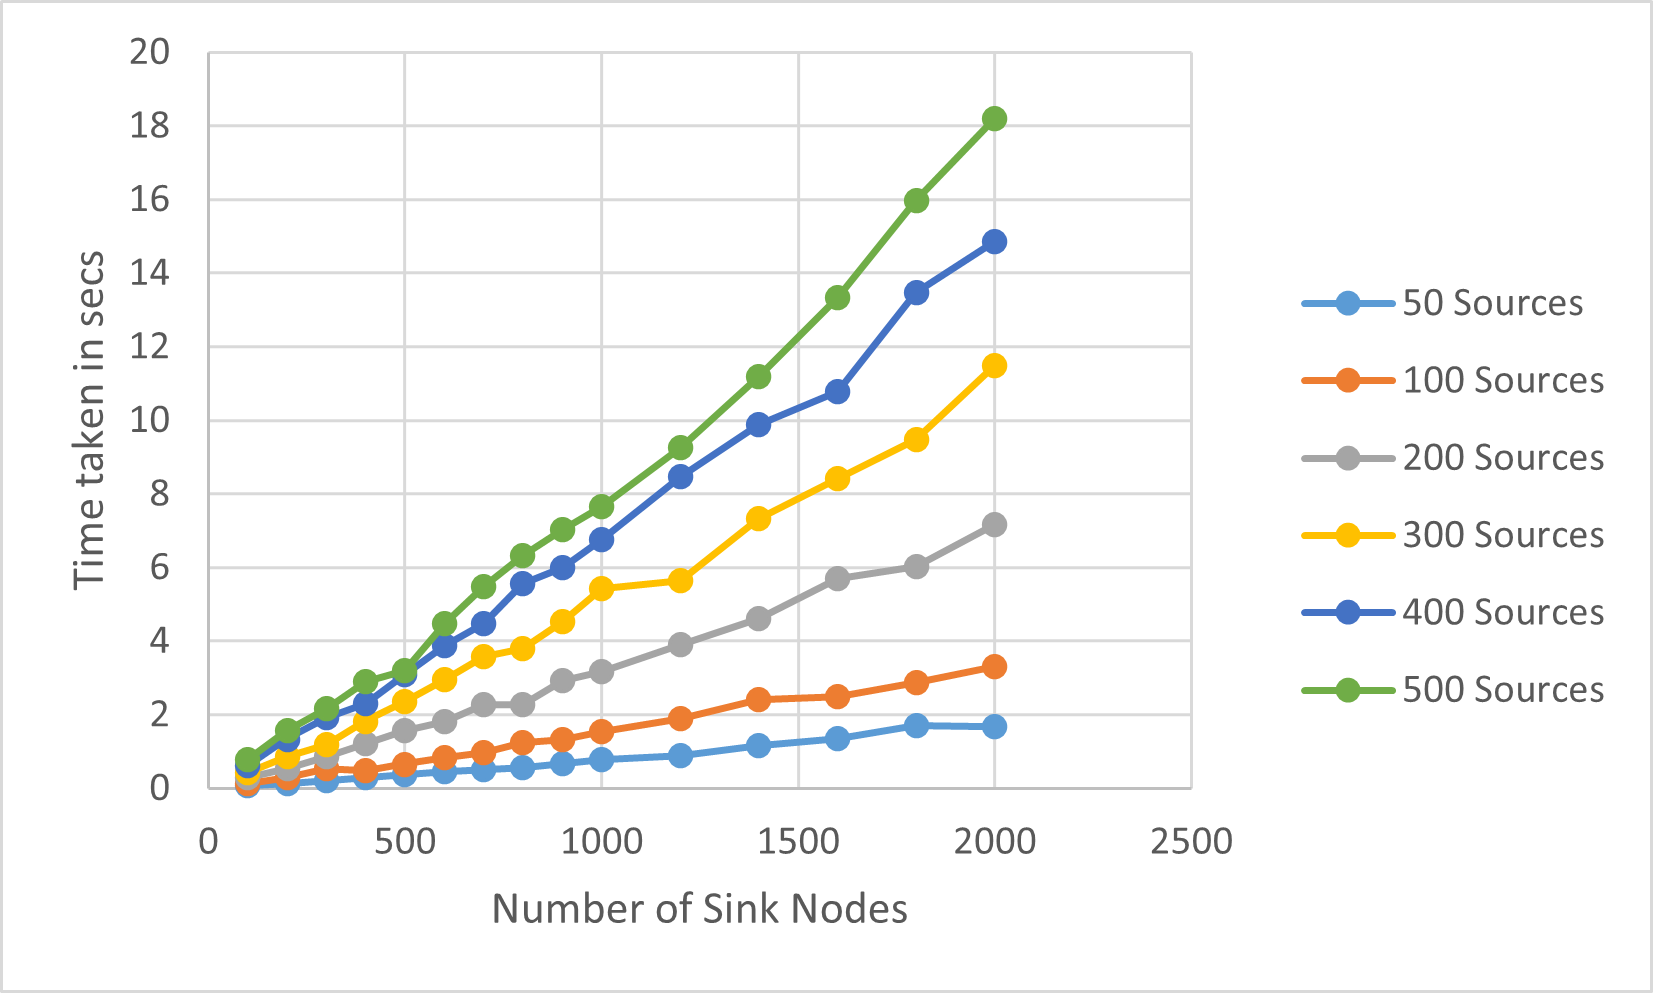
\includegraphics[width=0.9\linewidth]{lp.png}
  \caption{$network\_simplex$ function}
  \label{fig:sub2}
\end{subfigure}
\caption{Performance of Networkx Library }
\label{fig:test}
\end{figure}
We also discovered that another function which is implementation of Capacity Scaling Minimum Cost Flow function can also be used for solving this problem. 
\subsection{Other Libraries}
The prototype made with Boost Graph library gave us similar runtime as python code. But as python codes are inherently slow due to interpreted nature there is some issue with the prototype. Hence, we need to work on redefining the prototype. 

While working with LEMON prototype we got in conversation with Prof. Péter Kovács, who is major contributor in the library\cite{DEZSO201123}. We found lack of parallelized implementations of the algorithms which can significantly reduce improve the performance. 

We observed that, while executing programs only 1 core was getting utilised and was bottleneck in the overall performance. The runtime increased linearly with growth in source and sink nodes, which became impractical to operate on when cranked up to 10 thousands of node. We also discovered that there is scope to further optimize performance by adding parallelizing the current implementations. 

\section{Next Steps}
Our next objectives include:
\begin{itemize}
    \item Modifying Prototype with Boost Graph Library for optimal performance
    \item Implementing Prototype with LEMON library
    \item Measuring the execution time between the various steps of algorithm
    \item Implement Prototype with Capacity Scaling Minimum Cost Flow
    \item Adding parallel implementation for Cost Scaling Algorithm
\end{itemize}

\bibliographystyle{unsrtnat}
\bibliography{references}  %%% Uncomment this line and comment out the ``thebibliography'' section below to use the external .bib file (using bibtex) .


%%% Uncomment this section and comment out the \bibliography{references} line above to use inline references.
% \begin{thebibliography}{1}

% 	\bibitem{kour2014real}
% 	George Kour and Raid Saabne.
% 	\newblock Real-time segmentation of on-line handwritten arabic script.
% 	\newblock In {\em Frontiers in Handwriting Recognition (ICFHR), 2014 14th
% 			International Conference on}, pages 417--422. IEEE, 2014.

% 	\bibitem{kour2014fast}
% 	George Kour and Raid Saabne.
% 	\newblock Fast classification of handwritten on-line arabic characters.
% 	\newblock In {\em Soft Computing and Pattern Recognition (SoCPaR), 2014 6th
% 			International Conference of}, pages 312--318. IEEE, 2014.

% 	\bibitem{hadash2018estimate}
% 	Guy Hadash, Einat Kermany, Boaz Carmeli, Ofer Lavi, George Kour, and Alon
% 	Jacovi.
% 	\newblock Estimate and replace: A novel approach to integrating deep neural
% 	networks with existing applications.
% 	\newblock {\em arXiv preprint arXiv:1804.09028}, 2018.

% \end{thebibliography}

% https://github.com/zxqfl/flow/blob/master/src/lib.rs
% https://cp-algorithms.com/graph/min_cost_flow.html
% http://lemon.cs.elte.hu/pub/doc/latest/a00005.html
% https://joshkorn.com/flows.html
% https://en.wikipedia.org/wiki/Minimum-cost_flow_problem
\end{document}
